% Hybrid TLS 1.3 + PQC Handshake Sequence Diagram — Standalone TikZ
% Compile: pdflatex hybrid_tls_sequence_tikz.tex
% Include in main survey with 
\includegraphics{figures/hybrid_tls_sequence.pdf}

\documentclass[tikz,border=6pt]{standalone}
\usepackage{tikz}
\usetikzlibrary{arrows.meta,positioning,backgrounds}
\usepackage{xcolor}

\definecolor{cblue}{HTML}{003f87}
\definecolor{cred}{HTML}{c0392b}
\definecolor{cgreen}{HTML}{1a7a4a}
\definecolor{corange}{HTML}{e67e22}
\definecolor{cgray}{HTML}{7f8c8d}

\newcommand{\msg}[5]{%
  % #1=y, #2=x start, #3=x end, #4=label text, #5=color
  \draw[-{Latex[length=2.5mm]}, thick, color=#5]
    (#2,#1) -- (#3,#1)
    node[midway, above, font=\tiny, color=#5] {#4};
}

\begin{document}
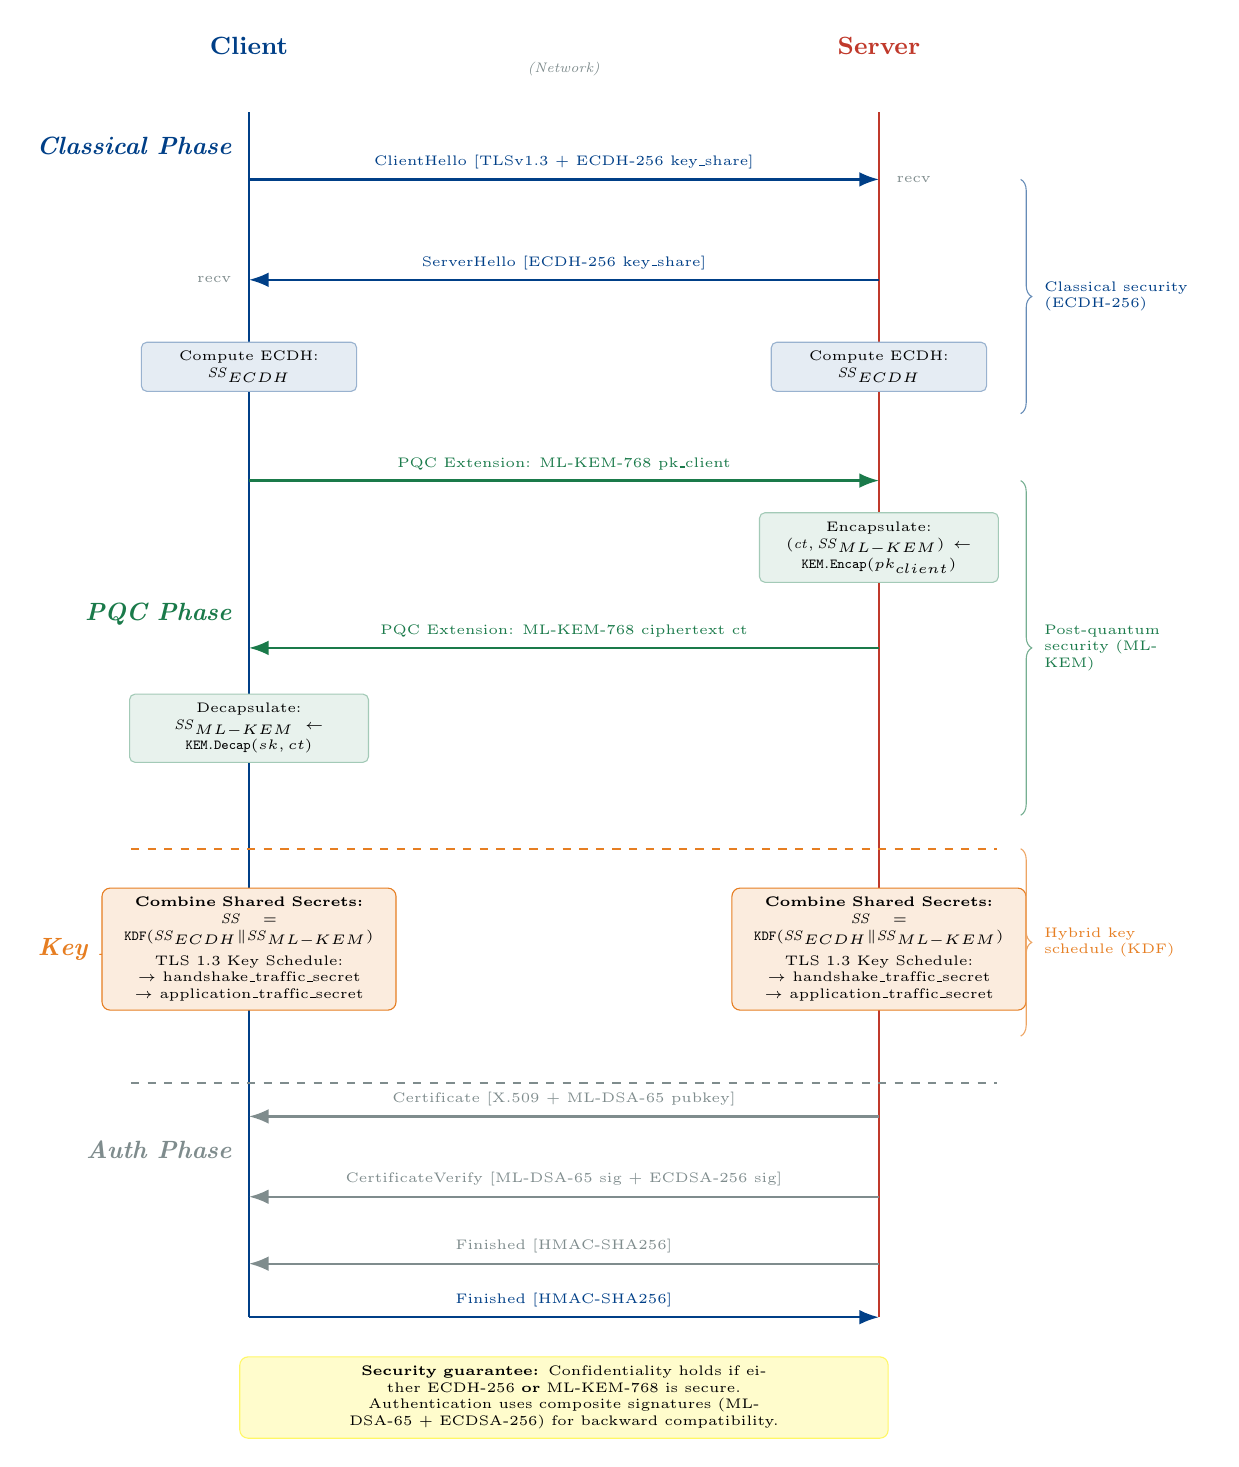
\begin{tikzpicture}[x=1cm, y=0.85cm]

% Lifelines
\node[font=\small\bfseries, color=cblue] at (0, 1.0)  {Client};
\node[font=\small\bfseries, color=cred]  at (8, 1.0)  {Server};
\node[font=\tiny, color=cgray]           at (4, 0.65) {\textit{(Network)}};

\draw[thick, color=cblue] (0,  0) -- (0, -18);
\draw[thick, color=cred]  (8,  0) -- (8, -18);

% Phase labels
\node[font=\footnotesize\bfseries\itshape, color=cblue, left=0.1cm] at (0, -0.5)
  {\small Classical Phase};
\node[font=\footnotesize\bfseries\itshape, color=cgreen, left=0.1cm] at (0, -7.5)
  {\small PQC Phase};
\node[font=\footnotesize\bfseries\itshape, color=corange, left=0.1cm] at (0, -12.5)
  {\small Key Derivation};
\node[font=\footnotesize\bfseries\itshape, color=cgray, left=0.1cm] at (0, -15.5)
  {\small Auth Phase};

% Classical messages
\msg{-1.0}{0}{8}{ClientHello [TLSv1.3 + ECDH-256 key\_share]}{cblue}
\node[font=\tiny, color=cgray, right=0.1cm] at (8,-1.0) {recv};

\msg{-2.5}{8}{0}{ServerHello [ECDH-256 key\_share]}{cblue}
\node[font=\tiny, color=cgray, left=0.1cm] at (0,-2.5) {recv};

\node[rectangle, fill=cblue!10, draw=cblue!40, font=\tiny, text width=2.5cm,
      align=center, rounded corners=2pt] at (0,-3.8)
  {Compute ECDH:\\$\mathit{SS}_\text{ECDH}$};
\node[rectangle, fill=cblue!10, draw=cblue!40, font=\tiny, text width=2.5cm,
      align=center, rounded corners=2pt] at (8,-3.8)
  {Compute ECDH:\\$\mathit{SS}_\text{ECDH}$};

% PQC messages
\msg{-5.5}{0}{8}{PQC Extension: ML-KEM-768 pk\_client}{cgreen}

\node[rectangle, fill=cgreen!10, draw=cgreen!40, font=\tiny, text width=2.8cm,
      align=center, rounded corners=2pt] at (8,-6.5)
  {Encapsulate:\\$(\mathit{ct}, \mathit{SS}_\text{ML-KEM}) \leftarrow$\\
   $\mathtt{KEM.Encap}(pk_\text{client})$};

\msg{-8.0}{8}{0}{PQC Extension: ML-KEM-768 ciphertext ct}{cgreen}

\node[rectangle, fill=cgreen!10, draw=cgreen!40, font=\tiny, text width=2.8cm,
      align=center, rounded corners=2pt] at (0,-9.2)
  {Decapsulate:\\$\mathit{SS}_\text{ML-KEM} \leftarrow$\\
   $\mathtt{KEM.Decap}(sk, ct)$};

% Combined key derivation
\draw[dashed, thick, color=corange] (-1.5,-11.0) -- (9.5,-11.0);

\node[rectangle, fill=corange!15, draw=corange, font=\tiny, text width=3.5cm,
      align=center, rounded corners=3pt] at (0,-12.5)
  {\textbf{Combine Shared Secrets:}\\
   $\mathit{SS} = \mathtt{KDF}(\mathit{SS}_\text{ECDH} \| \mathit{SS}_\text{ML-KEM})$\\[2pt]
   TLS 1.3 Key Schedule:\\
   $\rightarrow$ handshake\_traffic\_secret\\
   $\rightarrow$ application\_traffic\_secret};

\node[rectangle, fill=corange!15, draw=corange, font=\tiny, text width=3.5cm,
      align=center, rounded corners=3pt] at (8,-12.5)
  {\textbf{Combine Shared Secrets:}\\
   $\mathit{SS} = \mathtt{KDF}(\mathit{SS}_\text{ECDH} \| \mathit{SS}_\text{ML-KEM})$\\[2pt]
   TLS 1.3 Key Schedule:\\
   $\rightarrow$ handshake\_traffic\_secret\\
   $\rightarrow$ application\_traffic\_secret};

% Authentication
\draw[dashed, thick, color=cgray] (-1.5,-14.5) -- (9.5,-14.5);

\msg{-15.0}{8}{0}{Certificate [X.509 + ML-DSA-65 pubkey]}{cgray}
\msg{-16.2}{8}{0}{CertificateVerify [ML-DSA-65 sig + ECDSA-256 sig]}{cgray}
\msg{-17.2}{8}{0}{Finished [HMAC-SHA256]}{cgray}
\msg{-18.0}{0}{8}{Finished [HMAC-SHA256]}{cblue}

% Security annotations
\draw[decorate, decoration={brace,amplitude=4pt}, color=cblue!60]
  (9.8,-1.0) -- (9.8,-4.5)
  node[midway, right=5pt, font=\tiny, color=cblue, text width=2cm]
  {Classical security\\(ECDH-256)};

\draw[decorate, decoration={brace,amplitude=4pt}, color=cgreen!60]
  (9.8,-5.5) -- (9.8,-10.5)
  node[midway, right=5pt, font=\tiny, color=cgreen, text width=2cm]
  {Post-quantum\\security (ML-KEM)};

\draw[decorate, decoration={brace,amplitude=4pt}, color=corange!70]
  (9.8,-11.0) -- (9.8,-13.8)
  node[midway, right=5pt, font=\tiny, color=corange, text width=2cm]
  {Hybrid key\\schedule (KDF)};

% Security note
\node[rectangle, fill=yellow!20, draw=yellow!60, font=\tiny, text width=8cm,
      align=center, rounded corners=3pt] at (4,-19.2)
  {\textbf{Security guarantee:} Confidentiality holds if either ECDH-256 \textbf{or}
   ML-KEM-768 is secure.\\
   Authentication uses composite signatures (ML-DSA-65 + ECDSA-256) for
   backward compatibility.};

\end{tikzpicture}
\end{document}
